Le code de transformation complet étant assez long je vais ici expliquer à l'aide de graphiques les opérations pour transformer les éléments SimplePDL en éléments de réseau de pétri :\\

\subsection{WorkDefinition WD}
J'ai voulu modifier au minimum la structure des WD et des WS dont on avait les transformations avant l'ajout des ressources aux modèles.
Ainsi on assure une évolution simple des WD et WS.\\

On commence par une WorkDefinition WD. Avec les ressources en plus, une WD a besoin de savoir si des ressources sont disponibles pour pouvoir démarrer une activité.
\begin{itemize}
   \item On ajoute donc une place ressources\_available reliée à la transition start d'une WD.
   \item On ajoute également une place ressources\_wait (marquée à 1) pour indiquer que la WD est en attente de ressources
   \item Enfin on ajoute une place ressources\_returned reliée en sortie de la transition finish qui inque que la WD a fini d'utiliser les ressources
\end{itemize}

\vspace{1em}
On a donc ajouté 3 places et 2 arcs à notre WD. Voici un graphique récapitulatif :

\begin{figure}[h]
\centering
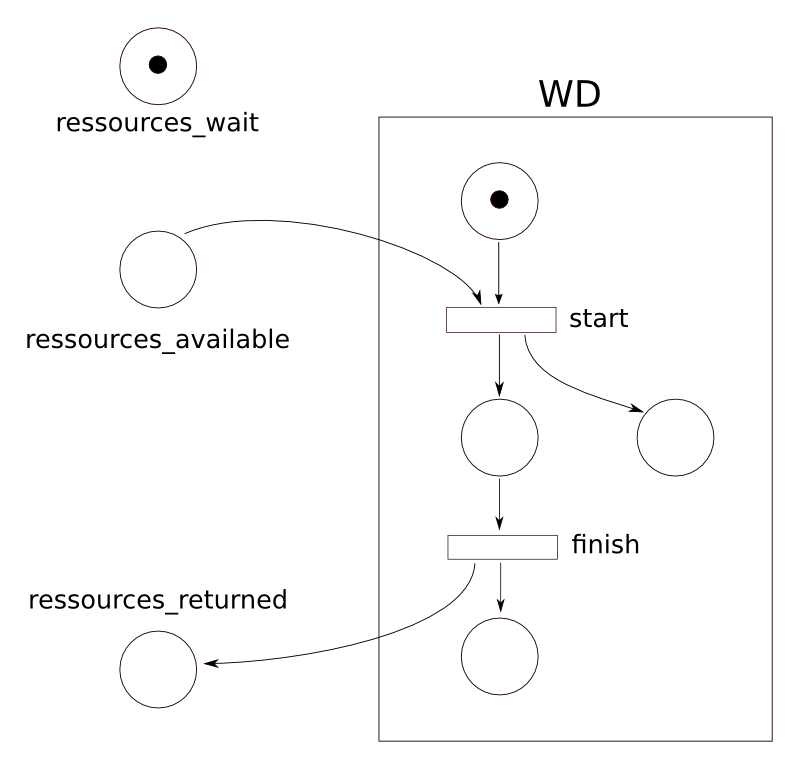
\includegraphics[width=0.6\textwidth]{../Images/WD2petri.png}
\label{WD2petri}
\caption{Transformation d'une WorkDefinition WD en réseau de pétri}
\end{figure}

\newpage
\subsection{NeedSet}
Je ne décris pas le besoins (Need) car il s'agit d'une simple place avec un marquage correspondant à "quantity".\\

Chaque ensemble de besoins (NeedSet) correspond à un ensemble constitué de :
\begin{itemize}
   \item une place "set" pour indiquer de quel NeedSet il s'agit
   \item 3 transition :
      \begin{itemize}
         \item "take" qui est reliée à chaque ressource nécessaire pour le NeedSet
         \item "makeAvailable" entre la place "set" du NeedSet et la place "ressources\_available" de la WD
         \item "return" reliée aux ressources qui vont être rendues
      \end{itemize}
   \item enfin les arcs qui vont bien (voir schéma)
\end{itemize}

\begin{figure}[h]
\centering
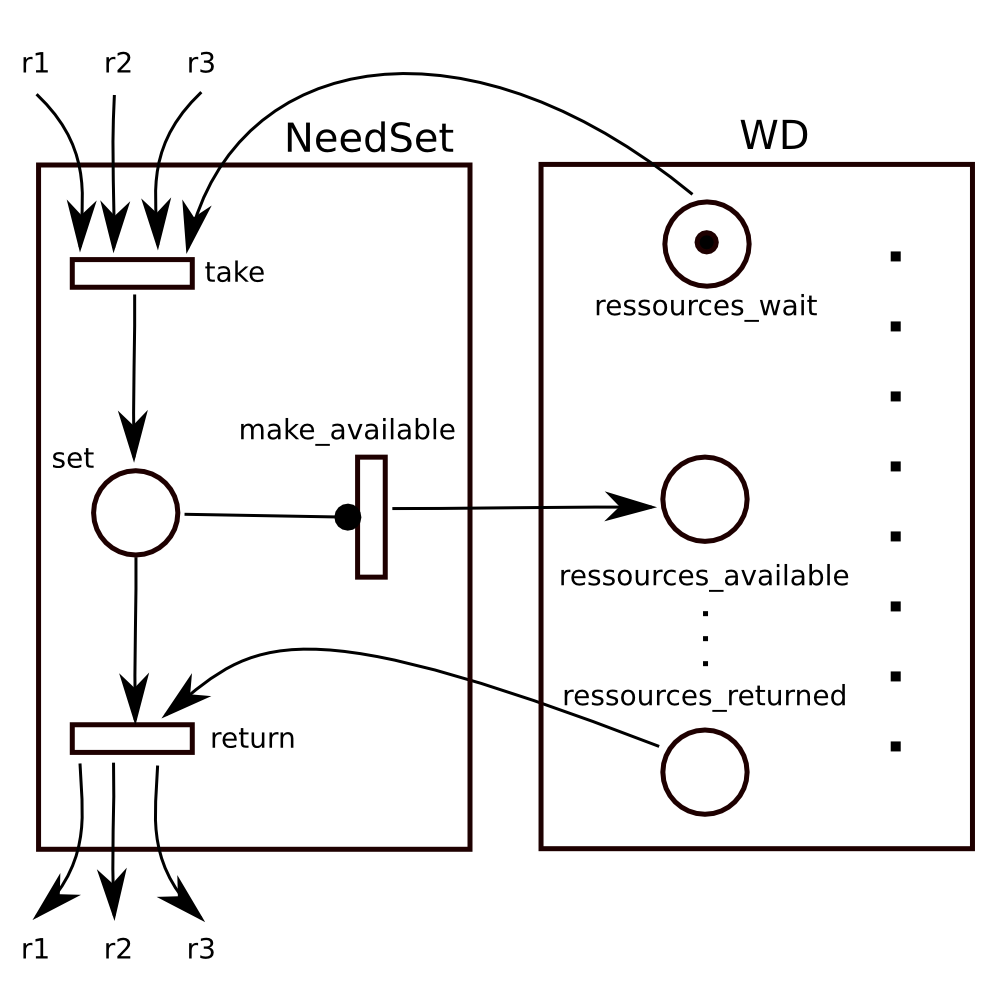
\includegraphics[width=0.6\textwidth]{../Images/NeedSet2petri.png}
\label{WD2petri}
\caption{Transformation d'un ensemble de besoins NeedSet en réseau de pétri}
\end{figure}

